\documentclass{standalone}
\usepackage{pgfplots}
\usepackage{tikz}


\newcommand{\gridCirc}[2]{
\addplot[data cs=polar,red,domain=0:360,samples=360,smooth,#2] (x,#1);
}

\newcommand{\constCirc}[4]{
\addplot[data cs=polar,red,domain=0:360,samples=#1+1,smooth,mark=*, only marks,#4] (x+#3,#2);
}


\begin{document}

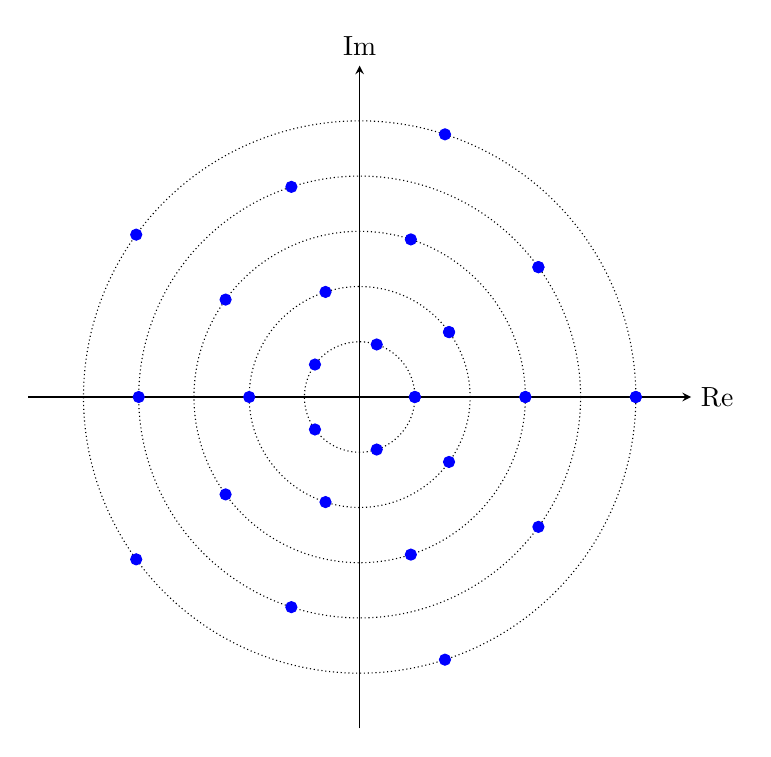
\begin{tikzpicture}
\begin{axis}[
  width = 10cm,
  height = 10cm,
  xlabel={$t$},
  axis x line=middle,  % Show only the x-axis
  axis y line=middle,    % Hide the y-axis
  xmin=-6, xmax=6,
  ymin=-6, ymax=6,  % Set ymax to 2
  xtick=\empty,
  ytick=\empty,
  xlabel = Re,
  ylabel = Im,
  xlabel style={
    right,
  },
  ylabel style={
    above,
  },
  legend style={draw=none,nodes={scale=0.4, transform shape}}
]

\gridCirc{1}{black, densely dotted}
\constCirc{5}{1}{0}{blue, fill=blue }

\gridCirc{2}{black, densely dotted}
\constCirc{5}{2}{36}{blue, fill=blue }

\gridCirc{3}{black, densely dotted}
\constCirc{5}{3}{0}{blue, fill=blue }

\gridCirc{4}{black, densely dotted}
\constCirc{5}{4}{36}{blue, fill=blue }

\gridCirc{5}{black, densely dotted}
\constCirc{5}{5}{0}{blue, fill=blue }


\end{axis}
\end{tikzpicture}

\end{document}